\documentclass[12pt, twoside]{article}
\usepackage[francais]{babel}
\usepackage[T1]{fontenc}
\usepackage[latin1]{inputenc}
\usepackage[left=1cm, right=1cm, top=1cm, bottom=1cm]{geometry}
\usepackage{float}
\usepackage{graphicx}
\usepackage{array}
\usepackage{multirow}
\usepackage{amsmath,amssymb,mathrsfs}

\begin{document}
\begin{flushright}
$2^{de}5$
\end{flushright}
\begin{center}
{\fbox{ \textbf{\Large{Mini Devoir Maison 1}}}}
\end{center}

\medskip

\textbf{NOM Pr�nom:} \ldots \ldots \ldots \ldots \ldots \ldots
\bigskip


\textit{Devoir � rendre pour le samedi 04 octobre 2008 sur feuille double grand
format. On pourra compl�ter la figure sur la photocopie qui est � rendre. La
clart� de la r�daction sera prise en compte.}


\bigskip

\textbf{Exercice}: \textit{Les constructions sont � faire sur la figure
ci-dessous.} 
\medskip


Sur la droite gradu�e de rep�re $(O,I)$, $B$ a pour abscisse $6$. Soit
$\mathcal{C}1$ le cercle de centre $B$ et de rayon $5$ et $\mathcal{C}2$ le cercle de diam�tre $[OB]$. 
On appelle $C$ l'un des points d'intersection du cercle $\mathcal{C}1$ et
$\mathcal{C}2$. Le cercle de centre $O$ et de rayon $OC$ not� $\mathcal{C}3$ coupe la droite r�elle au point $D$ d'abscisse $x$.

\medskip

\begin{enumerate}
  \item Que vaut $BC$?
  \item Montrer que $OBC$ est un triangle rectangle en $C$.
  \item \begin{enumerate}
          \item Calculer $OC$.
          \item En d�duire la valeur de $x$.
          \item Quelle est la nature de $x$ (la nature d'un nombre c'est le
          plus petit ensemble auquel il appartient)?
\end{enumerate}
\item  Tracer la m�diatrice $(d)$ de $[OI]$ (� la r�gle et au compas). Soit $A$ le point d'intersection de $[OI]$ et de $(d)$. 
        Que vaut l'abscisse de $A$? Quelle est la nature de ce nombre?

\item Soit E le point sur $(OI)$ d'abscisse $\frac{7}{3}$. Donner une m�thode
g�om�trique pour construire le point $E$ (� construire sur votre copie double).
Justifier votre construction.
\item Quelles difficult�s avez vous rencontr�es lors du contr�le sur table?

\end{enumerate}

\bigskip

\begin{center}
	  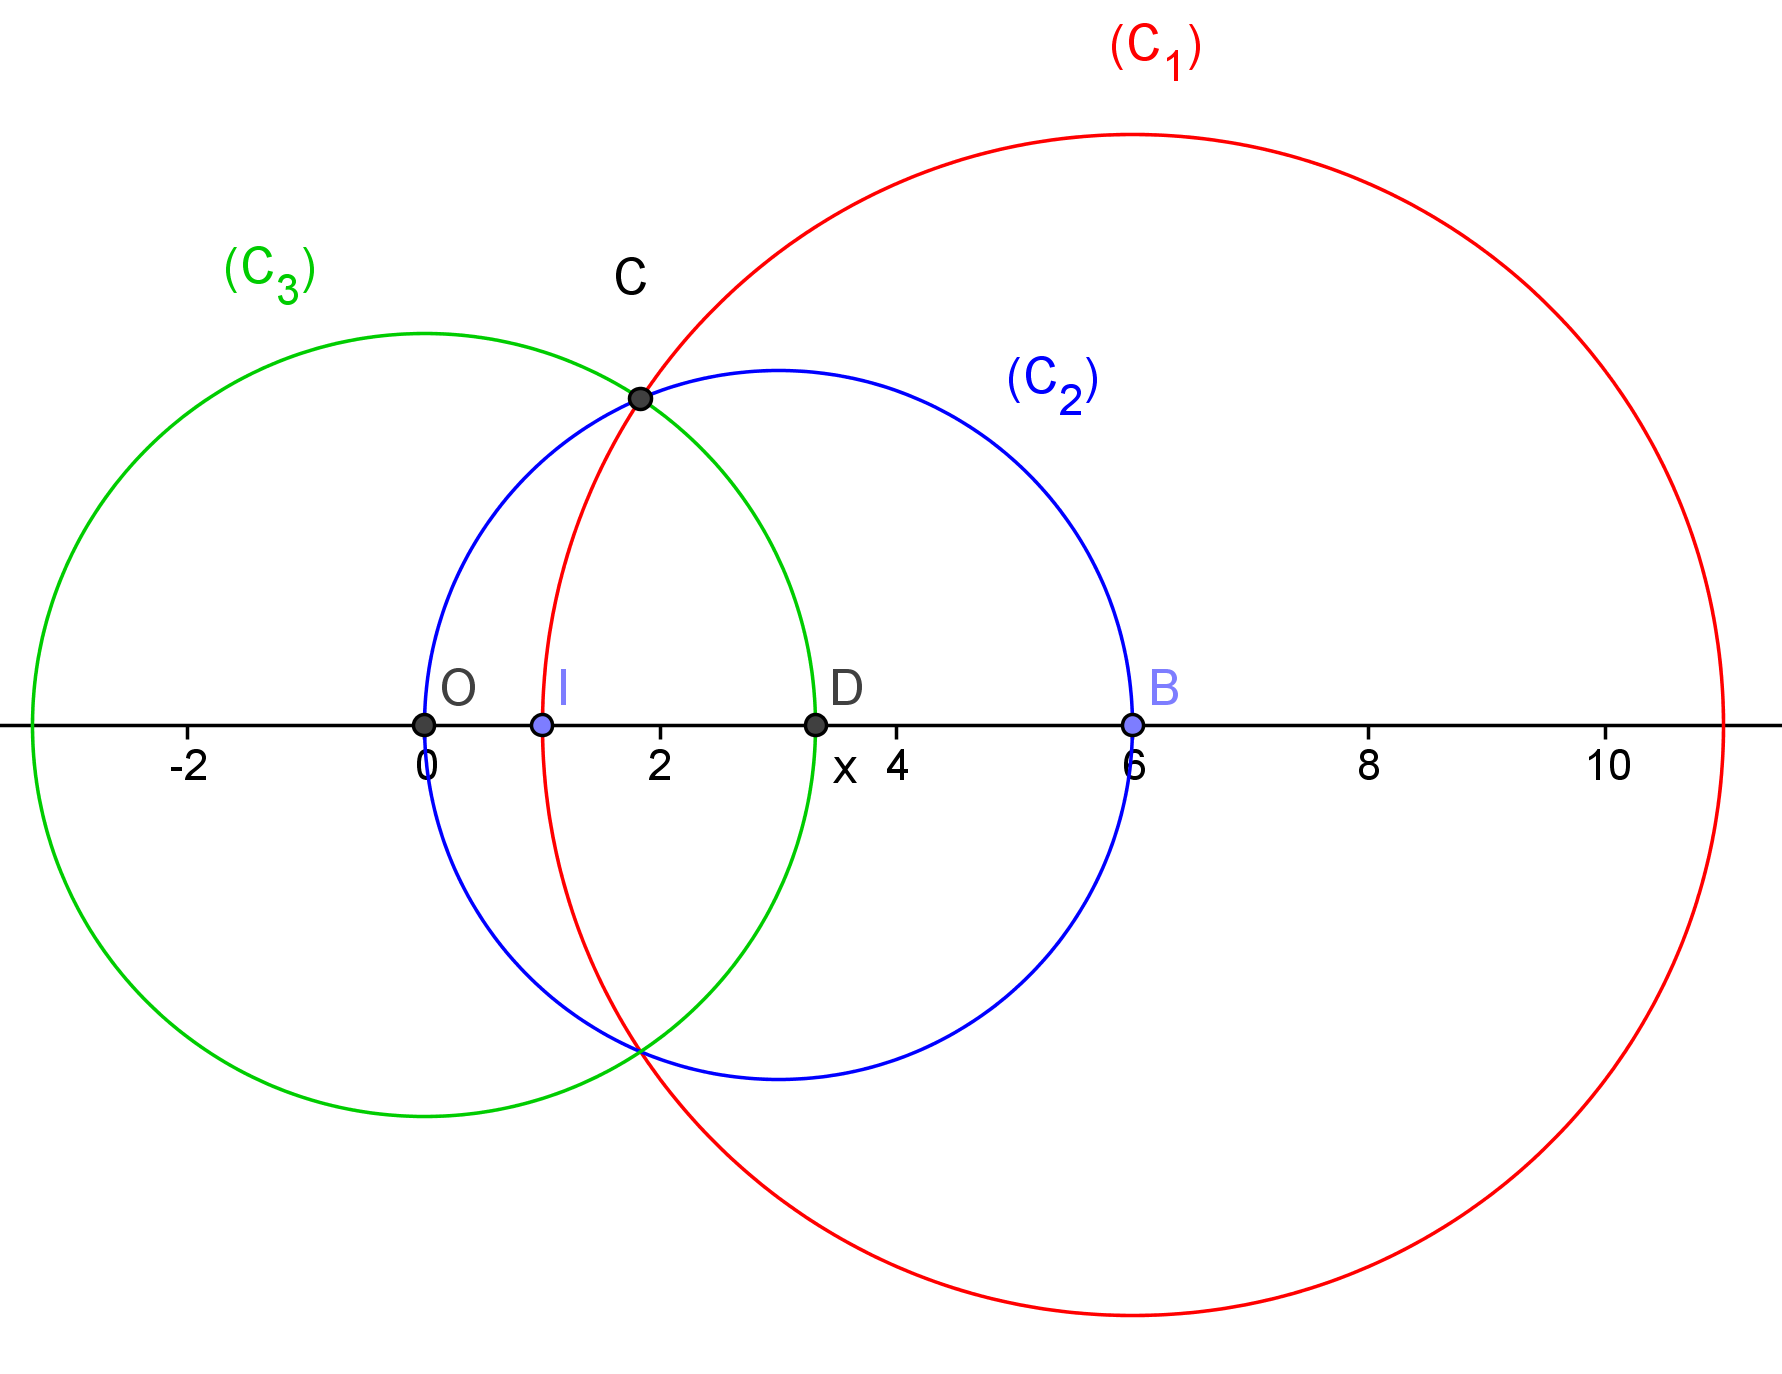
\includegraphics[width=12cm]{image/minidm1.png} 
\end{center}
\end{document}